\problemname{Uppställning}
En grupp med n barn, låt oss kalla dem A, B, C och så vidare, beslutar sig för att testa din tankeförmåga.
Utan att du ser dem ställer de upp sig på en rad.
Sen räknar vart och en av dem hur många av de barn som står till vänster som är längre än hen själv, och sedan likadant med dem som står till höger.
Var och en skriver ner dessa antal på en lapp som de ger till dig efter att ha frångått uppställningen.
Deras enkla uppmaning till dig är att tala om i vilken ordning de stod.

Ett exempel med fem barn visas i figuren.
A har ett längre barn (D) till vänster om sig och två (C och E) till höger.
B har tre längre barn till vänster om sig och ett till höger.
C har ett längre barn till vänster om sig men inget till höger och så vidare.
Informationen på lapparna kan sammanfattas så här:

\begin{figure}[h!]
  \centering

\begin{minipage}{.5\textwidth}
    \begin{tabular}[b]{|c|c|c|}
    \hline
      Barn&Vänster&Höger\\\hline
      A&1&2\\
      B&3&1\\
      C&1&0\\
      D&0&0\\
      E&2&0\\\hline
    \end{tabular}
\end{minipage}%
\begin{minipage}{.5\textwidth}
    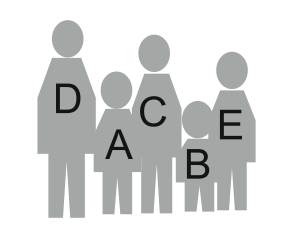
\includegraphics[scale=0.4]{uppstallning.png}
\end{minipage}

\end{figure}

Tyvärr klarade du inte nöten utan måste i hemlighet smyga iväg och skriva ett datorprogram som löser uppgiften.
För att underlätta för dig själv nästa gång barnen ansätter dig så vill du kunna variera både antalet barn (mellan 3 och 8, inklusive) och informationen på lapparna.
Du kan förutsätta att alla barn är olika långa och att de inte har gjort något misstag när de skrev lapparna.
Intressant nog finns det aldrig mer än en lösning.

\section*{Indata}
Första raden i indata består av ett heltal $n$ ($3 \le n \le 8$), antal barn.
Därefter följer $n$ rader med två heltal vardera: antal barn till vänster som är längre än barnet självt, och antalet till höger.

\section*{Utdata}
Skriv ut en rad med $n$ tecken som beskriver barnens uppställning, som en omkastning av bokstäverna \texttt{A}, \texttt{B}, \texttt{C}, etc.
